
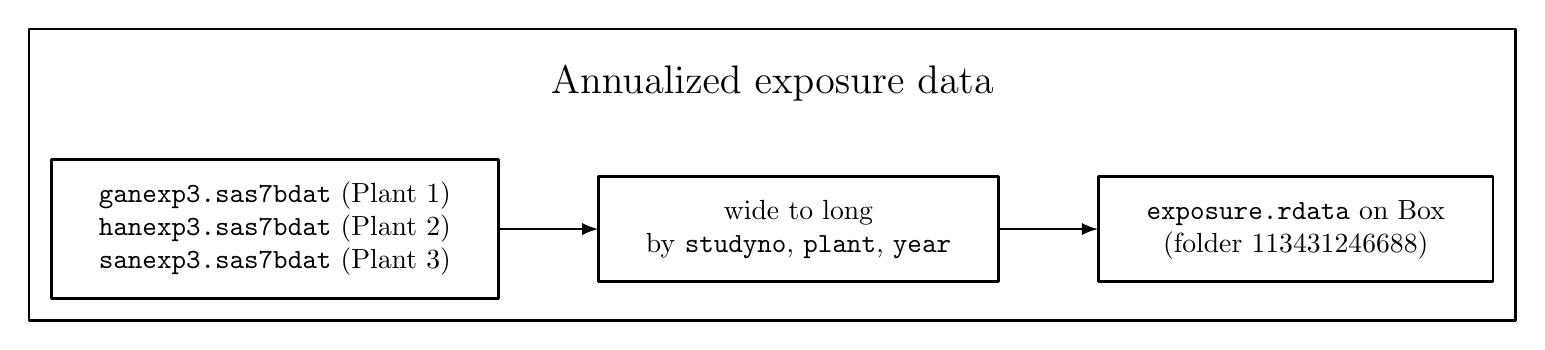
\begin{tikzpicture}[>=latex,line join=bevel,]
  \pgfsetlinewidth{1bp}
%%
\begin{scope}
  \pgfsetstrokecolor{black}
  \definecolor{strokecol}{rgb}{0.0,0.0,0.0}
  \pgfsetstrokecolor{strokecol}
  \draw (8.0bp,8.0bp) -- (8.0bp,113.0bp) -- (543.0bp,113.0bp) -- (543.0bp,8.0bp) -- cycle;
  \draw (275.5bp,93.5bp) node {\Large Annualized exposure data};
\end{scope}
  \pgfsetcolor{black}
  % Edge: exposure -> long
  \draw [->] (177.13bp,41.0bp) .. controls (185.58bp,41.0bp) and (194.18bp,41.0bp)  .. (212.89bp,41.0bp);
  % Edge: long -> final
  \draw [->] (357.23bp,41.0bp) .. controls (365.56bp,41.0bp) and (374.1bp,41.0bp)  .. (392.78bp,41.0bp);
  % Node: final
\begin{scope}
  \definecolor{strokecol}{rgb}{0.0,0.0,0.0}
  \pgfsetstrokecolor{strokecol}
  \draw (535.0bp,60.0bp) -- (393.0bp,60.0bp) -- (393.0bp,22.0bp) -- (535.0bp,22.0bp) -- cycle;
  \draw (464.0bp,41.0bp) node {\begin{tabular}{c} 
						\texttt{exposure.rdata} on Box \\						({folder 113431246688})
						\end{tabular}};
\end{scope}
  % Node: long
\begin{scope}
  \definecolor{strokecol}{rgb}{0.0,0.0,0.0}
  \pgfsetstrokecolor{strokecol}
  \draw (357.0bp,60.0bp) -- (213.0bp,60.0bp) -- (213.0bp,22.0bp) -- (357.0bp,22.0bp) -- cycle;
  \draw (285.0bp,41.0bp) node {\begin{tabular}{c} 
						wide to long \\						by \texttt{studyno}, \texttt{plant}, \texttt{year}
						\end{tabular}};
\end{scope}
  % Node: exposure
\begin{scope}
  \definecolor{strokecol}{rgb}{0.0,0.0,0.0}
  \pgfsetstrokecolor{strokecol}
  \draw (177.0bp,66.0bp) -- (16.0bp,66.0bp) -- (16.0bp,16.0bp) -- (177.0bp,16.0bp) -- cycle;
  \draw (96.5bp,41.0bp) node {\begin{tabular}{c} 
						\texttt{ganexp3.sas7bdat} (Plant 1) \\						\texttt{hanexp3.sas7bdat} (Plant 2) \\						\texttt{sanexp3.sas7bdat} (Plant 3) \\						\end{tabular}};
\end{scope}
%
\end{tikzpicture}

